\documentclass[12pt]{article}
\usepackage{listings}
\usepackage{graphicx}
\usepackage{amsmath,amsfonts,amssymb}
\graphicspath{ {images/} }
\usepackage[numbers, square, sort]{natbib}
\usepackage[left=1in, top=1in, right=1in, bottom=1in, nohead]{geometry}
\usepackage{hyperref}

\usepackage[toc,page]{appendix}
\hypersetup{colorlinks=true, linkcolor=red, citecolor=blue, urlcolor=cyan}
\newcommand*{\Appendixautorefname}{appendix}
%new commands for l-th group etc
\newcommand{\grpidx}{l}
\usepackage[svgnames]{xcolor}
\newcommand{\djm}[1]{\textcolor{red}{(DJM: #1)}}
\newcommand{\norm}[1]{\left\lVert #1 \right\rVert}
\usepackage{algorithm,algorithmic}
\renewcommand{\algorithmiccomment}[1]{\hfill $\rhd$ #1}
\def\algorithmautorefname{Algorithm}

\lstset{language=R,
		basicstyle=\small\ttfamily,
		stringstyle=\color{DarkGreen},
		otherkeywords={0,1,2,3,4,5,6,7,8,9},
		morekeywords={TRUE,FALSE},
		deletekeywords={data,frame,length,as,character},
		keywordstyle=\color{blue},
		commentstyle=\color{DarkGreen}
		}

\newcommand{\pkg}[1]{{\normalfont\fontseries{b}\selectfont #1}}
\let\proglang=\textsf
\let\code=\texttt



\title{Comparing Algorithms for the Sparse Group Lasso}
\author{Aaron Cohen}


\begin{document}
    \maketitle
    \begin{abstract}
        The sparse group lasso is a high-dimensional regression technique that is useful for problems whose covariates have a naturally grouped structure, and where sparsity is encouraged at both the group and individual covariate level. In this paper we discuss two algorithms for this optimization problem, as well as their implementation in Fortran as part of a new R package. This R package is an advance over existing packages, as it is the only one that solves this problem in a sufficiently fast computation time for truly high-dimensional situations.
    \end{abstract}

\section{Introduction}
\label{Sec:intro}
The lasso is ``a regression analysis method that performs both variable selection and regularization,'' which uses an $l1$ penalty \citep{tibshirani1996regression} to select a subset of predictors to be nonzero. The minimization problem is of the form
\[
\min_{\beta} \frac{1}{2}\norm{y-X\beta}_2^2 + \lambda \norm{\beta}_1,
\]
where $X$ is an $n$ by $p$ data matrix, $\beta$ is the unknown coefficient vector, and $\lambda$ is a hyperparameter that enforces the regularization/variable selection. In this problem it is assumed that the response $y$ is linearly related to the predictors (the columns of the data matrix $X$), with the goal being to estimate the coefficient vector $\beta$ responsible for this linear relationship. In general it will return a solution with some nonzero entries in the $\beta$ vector, and the rest zero.

A variant of this, the group lasso \citep{yuan2006model} is appropriate when there is a natural grouping structure for the coefficients; that is, we assume that the vector of coeffiecients is partitioned into groups, or subvectors, and, by analogy with regular lasso regression, only a few of the groups are active, i.e., have nonzero coefficients. The group lasso thus performs regularization that has the effect of discarding groups of predictors rather than the predictors themselves; it is of the form 
\[
\min_{\beta}\frac{1}{2}\norm{y-\sum_{l=1}^mX^{(l)}\beta^{(l)}}_2^2 + \lambda\sum_{l=1}^m\sqrt{p_l}\norm{\beta^{(l)}}_2.
\]
Note that the grouping structure is explicit in the above equation: the vector of coefficients, $\beta$, is thought of as a concatination of the coefficient subvectors of the various groups $\beta^{(l)}$, and similarly the data matrix $X$ is the concatination of submatrices, each submatrix $X^{(l)}$ being composed of the columns that correspond to the particular group. Thus the first part of the equation, $y-\sum_{l=1}^mX^{(l)}\beta^{(l)}$, is identical to the more simply-written equation $y-X\beta$, but is written with this partition in mind. 

The second part of the equation, however---$\sum_{l=1}^m\sqrt{p_l}||\beta^{(l)}||_2$---is different than the corresponding part in the original lasso equation. Rather than being an $l1$ norm of the vector $\beta$, it is a sum of the (non-squared) $l2$ norms of the coefficient vectors of the various groups. It is interesting to note that it is the non-differentiability of this expression at $0$ that accounts for the group-discarding property of the problem, similar to how the $l1$ norm's non-differentiability at 0 is responsible for the discarding property of coefficients in the original lasso. 

As with the original lasso equation, there is only a single tuning parameter $\lambda$, whose value determines the strength of regularization. Within the second summation are the relative weights of the groups, $p_l$, though these are usually determined by the size of the corresponding groups, and so in the rest of this paper this notation is suppressed from the equations.

Finally, in a group-structured problem as above, it may be desirable to enforce sparsity, not only among the groups, but also within the groups. The sparse group lasso \citep{simon2013sparse} does this by solving the following minimization problem
\begin{equation}
  \label{eq:sparsegl}
\min_{\beta}\frac{1}{2}\norm{y-\sum_{l=1}^mX^{(l)}\beta^{(l)}}_2^2 + (1-\alpha)\lambda\sum_{l=1}^m||\beta^{(l)}||_2+\alpha\lambda||\beta||_1.
\end{equation}
This equation is very similar to that of the group lasso, and in fact one sees that the only difference is that it adds a second regularization term, the overall $l1$ norm of the full $\beta$ vector, which we first saw in the original lasso formulation.  There is now a second tuning parameter $\alpha$, which controls the relative emphasis of intra- vs inter- sparsity in the predictors.

The sparse group lasso, like the other two lassos, does not have a closed form solution and thus relies on computational algorithms, which may be very intensive for large datasets and/or many values of $\lambda$. The rest of this paper therefore concerns the mitigation of this issue, in particular the following question: if we are solving the sparse group lasso, not for a single value of the tuning parameter $\lambda$ but a whole parameter space---in this context, a range of values $(\lambda_1,\dots \lambda_S)$--- can we shorten the total computational time by making use of the already-computed solution at previous $\lambda$'s in the parameter space to speed up computation at a given $\lambda$?

In this paper we make use of a heuristic called the Strong Rule \citep{tibshirani2012strong} to help solve this problem, with some success. The strong rule uses the solution at the previous $\lambda_{s-1}$ to predict which groups will remain inactive upon solution at the current $\lambda_s$, and discards those groups before entering into the algorithm. If a significant number of groups are thrown out before entering the algorithm, convergence time can improve significantly.

The \texttt{R} package we have create has two algorithms, both using the strong rule, but in slightly different ways: the \textbf{three-step algorithm} and the \textbf{four-step algorithm}. Although they perform similarly for the simulated data set used in later sections of this paper, it is suspected that they will each be useful for different scenarios, depending on the size of the data, size of the predictors, and the true underlying group structure. This is explored in the last section before the conclusion.

%In this paper we consider solving the sparse group lasso for a whole range of parameters $(\lambda_1,\dots \lambda_n)$ rather than a single value, and a computational problem presents itself:  can we speed up the algorithm at a  given $\lambda_i$ by utilizing the solution at the previous $\lambda_{(i-1)}$? A heuristic solution to this, used in the present paper, is the Strong Rule \citep{tibshirani2012strong}, which predicts which predictor (groups) will remain zero at the solution for $\lambda_i$ and throws them out. If a significant number of groups are thrown out before entering the algorithm, convergence time can iprove significantly.

There are already two other existing \texttt{R} packages that perform group lasso, \pkg{gglasso} and \pkg{sgl}. The advantage of our package over those two are as follows: the sgl package has sparsity, but does direct coordinate descent and does not have a heuristic like the strong rule, so it does not take advantage of such a computational speedup. Because of this, \pkg{sgl} is too slow to be of use in analyzing the high-dimensional problems that occur commonly, for example in genetic applications.

The \pkg{gglasso} package, on the other hand, incorporates such a rule and is computationally fast, but does not incorporate within-group sparsity (i.e., it performs group lasso, not sparse group lasso). When this package is used on a grouped dataset, the solution will have some active groups and some inactive, but within an active group, generally all the coefficients will be nonzero. Our contribution, then, is to provide a package that performs sparse group lasso, and is faster than existing algorithms. The algorithms for this package are written in Fortran, and are based on the algorithm from the gglasso package.

In section 2, we describe the algorithm in detail, paying particular attention to the strong rule. In section 3, we show how to use the package, running through an example with simulated data. In section 4, we compare our package to the other existing sgl packages, and also compare the two variants of our algorithm with each other.

\section{Methodology}
\label{Sec:meth}

\subsection{Overview of the algorithm}

There is no closed-form solution to the optimization problem in \autoref{eq:sparsegl} above, so we need a numerical algorithm to find the optimal solution. The problem defined by \autoref{eq:sparsegl} is convex, since the expression is a sum of convex functions and the feasable set is convex, so there is an optimal solution, and a variety of methods may be used one.

Our package has two different algorithms to accomplish this, which we refer to as the \textbf{three-step} and \textbf{four-step} algorithms. The general framework for both of our algorithms is based on a block-wise coordinate descent algorithm (see \citep{yang2015fast, simon2013sparse}). What this means is that we loop over the groups and, for a given group, update only those variables while holding all other groups constant. In particular, we will use a majorization-minimization coordinate descent scheme; the term 'majorization' comes from the idea that, instead of using the exact equation to determine the step size and direction in every update step, we update according to a simpler expression than \autoref{eq:sparsegl} that majorizes, or bounds from above, the expression we want to solve for. This is explained in more detail in the following paragraph.

For the rest of this section, we will focus on a particular group $k$. We hold the coefficients for all other groups fixed, and find an appropriate update step for group $k$. We note here that, because the loss function in \autoref{eq:sparsegl} is differentiable and the penalty terms are convex and separable (i.e., they can be decomposed into a sum of functions each only involving a single group), a coordinate descent algorithm is guaranteed to converge to a global optimum \citep{tseng2001convergence}.

To begin with, we will introduce some notation. Let 

\[
r_{(-k)} = y - \sum_{l \neq k} X^{(l)} \beta^{(l)}
\]
be the partial residual of $y$, where all the group fits besides that of group $k$ are subtracted from $y$. Since all groups besides group $k$ are held fixed, we don't need to consider the penalty terms corresponding to those fixed groups. So what we are really interested in minimizing is the following:

\begin{equation}
	\label{eq:sparsegroupk}
\frac{1}{2n} \norm{r_{(-k)}-X^{(k)}\beta^{(k)}}_2^2 + (1-\alpha)\lambda \norm{\beta^{(k)}}_2 + \alpha \lambda \norm{\beta^{(k)}}_1. 
\end{equation}
For ease of notation, we will suppress the superscript $(k)$ from $\beta^{(k)}$, with the understanding that we are really referring to only the $k$-th group of the coefficient vector. We will also define, using these terms, the unpenalized loss function

\[
\ell (r_{(-k)}, \beta) = \frac{1}{2n}\norm{r_{(-k)} - X^{(k)}\beta}_2^2, 
\]
so that our optimization problem for the $k$-th group becomes $\ell (r_{(-k)},\beta) + (1-\alpha)\lambda\norm{\beta}_2 + \alpha \lambda \norm{\beta}_1$, and we are interested in finding an optimal value, $\hat{\beta}$.

Any global minimum is determined by the subgradient equation, which is similar to a first-derivative test for minima, except the $\norm{\cdot}_2$ and $\norm{\cdot}_1$ penalty terms are non-differentiable at $0$; because of this, the (sub)differential for each coordinate in $\beta$ (i.e., $\beta^{(k)}$) is not a single value, but a range of possible values. For \autoref{eq:sparsegroupk} above, taking the subdifferential and setting equal to zero gives us the following condition that the minimum $\hat{\beta}$ needs to satisfy: 

\begin{equation}
  \label{eq:subgrad}
\frac{1}{n}X^{(k)T}(r_{(-k)} - X^{(k)}\beta) = (1-\alpha)\lambda u + \alpha \lambda v,
\end{equation}
where $u$ is the subgradient of $\norm{\beta}_2$ and $v$ is the subgradient of $\norm{\beta}_1$. The first is defined to be $\frac{\beta}{\norm{\beta}_2}$ if $\beta$ is a nonzero vector, and is any value in the set $\{ u : \norm{u}_2 \leq 1 \}$ otherwise; the second, $v$, is defined coordinate-wise as $v_j = sign(\beta_j)$ if $v_j \neq 0$, and is any value $v_j \in \{v_j : |v_j| \leq 1 \}$ otherwise.


At this point, it is possible to use \autoref{eq:subgrad} to derive an update step and develop a cyclical coordinate-wise algorithm, but it is too computationally expensive, involving repeated large-matrix multiplication (\citep{simon2013sparse}); instead we use the majorization-minimization idea discussed above.

Since the unpenalized loss $\ell (r_{(-k)}, \beta)$ is a quadratic function in $\beta$, it is equal to its second order Taylor expansion about any point $\beta_0$ in the parameter space---indeed, this is the definition of a function being quadratic. We thus start with the following equality for any given $\beta_0$ (recall that $\beta_0 = \beta_0^{(k)}$):  

\begin{equation}
\forall \beta,\ \ell(\beta) = \ell(\beta_0)+(\beta - \beta_0)^T\nabla \ell(\beta_0)+\frac{1}{2}(\beta - \beta_0)^T H (\beta - \beta_0),
\label{eq:TaylorExp}
\end{equation}

where the gradient $\nabla \ell$ is the first total derivative of $\ell$ (evaluated at $\beta_0$) and $H$, the Hessian, is the second total derivative. Note that we have again suppressed notation, $\ell(\beta) = \ell(r_{(-k)},\beta)$, since $\beta = \beta^{(k)}$ is the only variable. Recall that $\nabla$ is the vector of first partial derivatives of $\ell$ with respect to each coordinate of $\beta$, evaluated at $\beta_0$, and $H$ is a $p$x$p$ matrix of mixed partial derivatives of $\ell$. In this particular case, a short computation shows that the Hessian is simply written in terms of $X$: $H = X^TX$.

The matrix $X$ is, for the problems we are interested in solving, very large, and so computing $X^TX$, storing it in memory, and inverting, is going to be an issue, especially since we will be doing update steps many times. What we can do, and will do, is replace this matrix with a much simpler one, $tI$, a diagonal matrix with the value of $t$ selected to be such that this dominates the Hessian (in the sense that $tI - H$ is positive definite). For our algorithm we choose the largest eigenvalue of the Hessian and use that for $t$. We get the following inequality:



\begin{equation}
\forall \beta,\beta_0,\ \ell(\beta) \leq \ell(\beta_0)+(\beta - \beta_0)^T\nabla \ell(\beta_0)+\frac{1}{2t}(\beta - \beta_0)^T  (\beta - \beta_0).
\label{eq:dominate}
\end{equation}

We take the original minimization problem (\autoref{eq:sparsegroupk}) and replace the loss $\ell$ with the right-hand side of \autoref{eq:dominate}. Thus \autoref{eq:sparsegroupk} is now dominated (majorized) by the following expression
\begin{equation}
\label{eq:Meq}
M(\beta) = \ell(\beta_0)+(\beta - \beta_0)^T\nabla \ell(\beta_0)+\frac{1}{2t}\norm{\beta_0-\beta}_2^2+ (1-\alpha)\lambda\norm{\beta}_2+\alpha\lambda\norm{\beta}_1,
\end{equation}
which no longer involves the large matrix multiplication that using the original loss function would have confronted us with. 

The optimal value $\hat{\beta}$ for $M(\beta)$ is determined by its subgradient equation, which is similar to that of \autoref{eq:subgrad}:

\begin{equation}
\frac{1}{t} (\beta - (\beta_0 - t\nabla \ell)) +(1-\alpha)\lambda u + \alpha \lambda v = 0,
\end{equation}
with $u$ and $v$ as before. If we solve this for $\beta$ in terms of $\beta_0$, paying close attention to the conditions for the subdifferentials when $\beta$ is and isn't $0$, we get the following equation:
\begin{equation}
\hat{\beta} = U(\beta_0) =
\left(1-\frac{t(1-\alpha)\lambda}{\norm{S(\beta_0-t\nabla \ell(\beta_0),\ t\alpha\lambda)}_2}\right)_+ S(\beta_0-t\nabla \ell(\beta_0),t\alpha\lambda),
\label{eq:updateStep}
\end{equation}
where $S$ is the coordinate-wise soft threshold operator, defined by a vector $\gamma$ and scalar $b$ according to
\begin{equation}
\label{softthresh}
(S(\gamma,b))_j = sign(\gamma_j)(|\gamma_j| - b)_+,
\end{equation}
i.e., for each coordinate in the vector, it shrinks that coordinate in magnitude by the amount $b$, and sets it to zero if the magnitude of that coordinate was smaller than $b$ to begin with.



\autoref{eq:updateStep} defines the update step at a given group $k$, via $\beta \leftarrow U(\beta)$. At a point $\beta_{old} = \hat{\beta}^{(k)}_{old}$, we find the convex function $M$ that majorizes the objective function--centered at that $\beta_{old}$--and choose the new value of beta to be the minimizer of majorized function, $\beta_{new} = U(\beta_{old})$. This update step has the advantage that it is easy to compute, and is guaranteed to converge to the optimum $\hat{\beta} = \hat{\beta}^{(k)}$ for that given group.  


By examining the update step we see that it is possible for the whole group to be set to zero (made inactive) because of the threshold operator $()_+$ in the first part of the expression, and it is possible also for individual components of $\beta^{(k)}$ to be zeroed out from the coordinate-wise threshold $S()$. From this it is seen that this update step tends to enforce sparsity at both the group and individual level.

Both of the algorithms in the \pkg{sparsegl} package use the update step $U$ in \autoref{eq:updateStep}, iterating over all the groups and performing one update per pass. Since the partial residual $r_{(-k)}$ is used in $U$ (via $\ell$), we note that, for a given group $k$ at a given point in the cycle, the update $\beta^{(k)} \leftarrow U(\beta^{(k)})$ uses the new values of $\beta^{(1)}, \dots \beta^{(k-1)}$ and the old values for the subsequent $\beta^{(k+1)},\dots \beta^{(m)}$.

Because the optimization problem is convex, with differentiable loss and separable penalty, it can be shown that this type of blockwise coordinate descent algorithm is guaranteed to converge to the optimal solution for the full vector $\hat{\beta}$. That is, it does not get `stuck' at any inflection points or local minima. Therefore, if that was all the algorithm did, there would be no need to check the KKT conditions for optimality. 

However, our algorithms both make use of the sequential strong rule, a heuristic that predicts, before computation, which groups will remain inactive, and discards them; this results in significant computational savings, but because this pre-processing prediction is not always correct, we will need to do a KKT check \citep{boyd2004convex} after convergence to make sure the initial prediction was accurate. This is described in the next section.

\subsection{KKT Check and the Strong Rule}

As mentioned above, the strong rule \citep{tibshirani2012strong} is easy and fast to perform, discarding large numbers of predictors before computation, but it is not guaranteed to be correct, so it becomes necessary to double-check the solution after convergence, to make sure active groups were not accidentally discarded. 

The version of the strong rule used here is called the \textbf{sequential strong rule}; it makes use of the fact that we are solving for a sequence $\{\lambda_1 \geq \lambda_2 \geq \dots \ ,\ \lambda_S\}$ of lambda parameters, rather than a single value. At each $\lambda_s$, we rely on the fact that we have solved the problem for the previous $\lambda_{s-1}$, and use this information to quickly discard many predictors. Without loss of generality, for the rest of this section assume that the problem has already been solved for $\lambda_{s-1}$.



The motivation for the strong rule comes from the KKT stationarity condition, which is similar to the first derivative test for minima \citep{boyd2004convex}. Explicitly, this is the condition that the subdifferential equations (see \autoref{eq:subgrad}) are satisfied at the proposed minimum $\hat{\beta} =\hat{\beta}(\lambda_s)$. This is the necessary and sufficient condition for a global optimum. Note that we will be emphasizing the dependence of $\hat{\beta},\ r_{(-k)}$, and so forth, on $\lambda$ in this section.
 
From \autoref{eq:subgrad} we derive an inequality that is equivalent to the KKT stationarity condition in the case that $\hat{\beta}^{(k)}=0$. Because the algorithm is guaranteed to converge to the optimum for all groups on which it is run, we only need to check the condition for the discarded groups, i.e., those that we have preassigned $\hat{\beta}^{(k)} = 0$ (at a given $\lambda$). 

First, if $\hat{\beta}^{(k)}=0$ then the subgradient equations reduce to the following:

\begin{equation}
\label{eq:subgradreduced}
X^{(k)T}r_{(-k)}/n - \alpha \lambda v = (1-\alpha) \lambda u,
\end{equation}
where $u$ and $v$ are the subdifferentials of $\norm{\beta^{(k)}}_2$ and $\norm{\beta^{(k)}}_1$, as in section 2.1. We claim that if the following inequality

\begin{equation}
\label{eq:kkt}
\norm{S(X^{(k)T}r_{(-k)}/n,\ \alpha\lambda)}_2 \leq (1-\alpha)\lambda
\end{equation}
is satisfied (with $S$ the soft-threshold operator from section 2.1), then $\hat{\beta}^{(k)}=0$ is the optimum for that group at that particular lambda. In other words, this inequality is equivalent to the kkt stationarity condition for inactive groups.

The proof is as follows: denote $\gamma = X^{(k)T}r_{(-k)}/n$, and define $v_j = sign((\gamma)_j)$ if $|\gamma_j| > \alpha \lambda$, and $v_j = \frac{\gamma_j}{\alpha \lambda}$ otherwise. Then 
\[
\gamma - \alpha \lambda v = S(\gamma,\alpha \lambda).
\]
Next, define $u = S(\gamma,\alpha \lambda)/(1-\alpha)(\lambda)$. From these two definitions it follows that \autoref{eq:subgradreduced} is satisfied, but not necessarily by elements of the subdifferentials. But if \autoref{eq:kkt} is also satisfied, then $u$ is a subgradient of $\norm{\beta^{(k)}}_2$, and $v$ a subgradient of $\norm{\beta^{(k)}}_1$, evaluated at $\beta^{(k)}=0$.

We have derived the KKT condition for the $k$-th group to be $0$. We will now derive and explain the strong rule, which is based on this inequality. At this point it will be helpful to make explicit the dependence of these expressions on $\lambda$. First, for each group $k$ we define a function of $\lambda$:

\begin{equation}
c_k(\lambda) = S(X^{(k)T}r_{(-k)}(\lambda)/n,\ \alpha\lambda).
\end{equation}
So for example \autoref{eq:kkt} becomes $\norm{c_k(\lambda)}_2 \leq (1-\alpha)\lambda$. There is a different function for every group $k$. Note that, since $r_{(-k)}$ involves $\hat{\beta}$, we needed to have actually solved the optimization problem at $\lambda$ in order to compute $c_k(\lambda)$.

It is natural to consider the properties such a function would have. These functions are continuous, for example, as the solution to the optimization problem \autoref{eq:sparsegl} varies continuously with its tuning parameter $\lambda$. We are now going to make an assumption about $c_k$, which seems unintuitive at first, and in fact is not always true, but is true often enough to be useful: we assume that $c_k(\lambda)$ is $(1-\alpha)$-Lipschitz, ie., that
\begin{equation}
\label{eq:lipschitz}
\forall \lambda,\ \lambda^{\prime}\ \  \ \norm{c_k(\lambda)-c_k(\lambda^{\prime})}_2 \leq (1-\alpha)\norm{\lambda - \lambda^{\prime}}_2.
\end{equation}
This is essentially saying that $c_k$ is not only continuous but does not vary 'too fast'; it is equivalent to saying that the function is differentiable almost everywhere and has bounded derivative.


We can finally define the \textbf{strong rule} check for discarding groups. Assume that the optimization problem has been solved for $\lambda_{s-1}$; then if the inequality
\begin{equation}
\label{eq:strong}
\norm{c_k(\lambda_{s-1})}_2 \leq (1-\alpha)(2\lambda_s - \lambda_{s-1})
\end{equation}
holds, then we discard group $k$ from the problem, before solving for $\lambda_s$. That is to say, when we move from $\lambda_{s-1}$ to $\lambda_s$, we first run this check on all groups, using the previously computed solution for $\hat{\beta}(\lambda_{s-1})$, and then move on to coordinate descent, using only those groups that failed this inequality.

This discarding rule is fast, using the previously computed solution and a simple inequality, and in practice it tends to accurately discard large numbers of groups. The reason why it works is as follows: assuming the Lipschitz condition on $c_k(\lambda)$, then if the strong rule is satisfied for $\lambda_s$, we get by the triangle inequality that
\begin{align*}
\norm{c_k(\lambda_s)}_2 &\leq \norm{c_k(\lambda_s) - c_k(\lambda_{s-1})}_2 + \norm{c_k(\lambda_{s-1})}_2 \\
&\leq (1-\alpha)(\lambda_{s-1} - \lambda_s) + (1-\alpha)(2\lambda_s - \lambda_{s-1})
=(1-\alpha)\lambda_s,
\end{align*}
which is exactly the KKT condition required for $\hat{\beta}^{(k)}(\lambda_s) = 0$, \autoref{eq:kkt}.

Note that the upper bound for the strong rule condition, the right-hand side of \autoref{eq:strong}, is smaller than the upper bound for the KKT condition inequality, i.e., $(1-\alpha)(2\lambda_s - \lambda_{s-1}) < (1-\alpha)(\lambda_{s-1})$, since $\lambda_{s} < \lambda_{s-1}$. We see from this that the strong rule condition, which is a condition on the subdifferential at $\lambda_{s-1}$, is stronger than the zero KKT condition at $\lambda_{s-1}$; the logic of the strong rule is that, if group $k$ satisfied the zero KKT condition at $\lambda_{s-1}$, with some wiggle room in the inequality, and if the function $c_k(\lambda)$ which characterizes the zero KKT condition does not change too much going from one lambda to the next, then the zero KKT will be satisfied for the next value $\lambda_s$.

Finally, we should reiterate that it is possible for the strong rule to make a mistake, the Lipschitz assumption is just that, an assumption. Because of this, it is critical that, after discarding some of the groups and running the algorithm on the others, the zero KKT condition is checked on all those discarded groups to make sure that the strong rule made the right decision, and that those groups are actually zero. Violators of the KKT condition should be put in 'active' status and the algorithm re-run with those groups included. The details of this are in the next section.

Now that we understand the KKT check and strong rule check on groups, we briefly discuss some notation which is used in the next section. In this section we defined a function $c_k(\lambda)$ that was parameterized by the group $k$ and taking in as an argument $\lambda$. We will change emphasis and define a function:
\[
\mathcal{S}_{\lambda}(A),
\]
that takes in a subset of the set of groups, $A$, and returns the set of all elements of $A$ which \textbf{fail} the strong rule check at $\lambda$. This is precisely the set of groups that we suspect of being active, that we should run the update step on. The reason why we want this notation is that it is a waste of time to run the strong rule check on those already known or suspected to be active. 

Similarly, we will define the function 
\[
KKT_{\lambda}(A)
\]
that takes in a  set of groups, and returns the subset of those elements of $A$ that \textbf{fail} the 0-KKT check, i.e. those elements $k \in A$ for which $\norm{c_k(\lambda)}_2 > (1-\alpha)\lambda$. Again, we do not need to check the KKT conditions for those groups on which the update step was run until convergence, so we will want to specify the subset of groups that we need to run the KKT check on after convergence of $U$.

\subsection{The three-step and four-step algorithms}




\begin{algorithm}[tb!]
  \caption{The Three-step Algorithm using the update step $U$ on suspected active groups via the Strong Rule, with a subsequent KKT check on inactive groups} 
  \label{alg:threeStep}
  \begin{algorithmic}
	\STATE 1. Initialize $\lambda = \lambda_s$. Run strong rule $\mathcal{S}_{\lambda}(\mathcal{E}^c)$, set $\mathcal{E} \leftarrow \mathcal{E}\cup\mathcal{S}_{\lambda}(\mathcal{E}^c)$    
    \STATE 2. Cycle through groups, run until convergence:
	\WHILE{$e>\epsilon$}
	\STATE {$e = 0$}	
	\FOR {$k=1 \dots m$}
	\STATE \textbf{if} $k \in \mathcal{E}^c$ \textbf{CYCLE}
	\STATE $e = max(e,\ \norm{\beta^{(k)} - U(\beta^{(k)}})$
	\STATE	$\beta^{(k)} \leftarrow U(\beta^{(k)})$
	\ENDFOR
	\STATE if $e < \epsilon$ end \textbf{while}
	\ENDWHILE
	\STATE 3. Run KKT check on inactive groups:
	\STATE \textbf{if} $KKT_{\lambda}(\mathcal{E}^c) \neq \emptyset$ \textbf{then}:
	\STATE $\mathcal{E} \leftarrow \mathcal{E}\cup KKT_{\lambda}(\mathcal{E}^c)$
	\STATE \textbf{goto} step 2
	\STATE \textbf{else}:
	\STATE Save $\hat{\beta} = \hat{\beta}(\lambda_s)$, \textbf{goto} step 1
  \end{algorithmic}
\end{algorithm}



There are two algorithms in our package that perform sparse group lasso: the three-step algorithm and the four-step algorithm. Both algorithms use the majorized coordinate-descent update step $U$ from section 2.1, and mainly differ in how they use the strong rule and how they store the active and potentially active groups. Before discussing these in detail, we need some notation.

First, recall from the end of the previous section that $\mathcal{S}_{\lambda}(A)$ is a function which performs the strong rule check on a set of groups $A$ at $\lambda$, and returns the set $A^{\prime}$ of groups in $A$ that fail the strong rule check. For each individual group in the set $A$, it checks the inequality in \autoref{eq:strong}. Recall that the strong rule check at a given $\lambda_k$ actually involves both $\lambda_{k}$ and $\lambda_{k-1}$; this is suppressed in this notation, with this understanding.

Similarly, the function $\textrm{KKT}_{\lambda} (A)$ performs the KKT check described in the previous section, and returns the subset $A^{\prime}$ of groups that fail the KKT check. The idea for both of these functions is to keep track of which groups are potentially active (nonzero) for the given $\lambda$. 

Both of these functions take in only a subset of the groups of coefficients, rather than being run on the whole set each time; this is to save time and reduce redundancy. It would not make sense to run a KKT check on those groups that are already known to be active (for the given $\lambda$), because the coordinate descent algorithm is guaranteed to converge for the groups on which is is run. Similarly for the strong rule check, it would be a waste of time to run that inequality on groups that are already known or suspected of being active, since the point of the strong rule check is to separate those suspected of being active from those that are not, and only updating the coefficient estimates for the suspected active groups.

We will keep track of active/potentially active groups with a set $\mathcal{E}$; this is the set of all groups that have failed the strong rule check, or have failed the KKT check, and it is precisely this set of groups that we perform the update step on until convergence. This set is ever-increasing, that is, if a group fails the strong rule or KKT check at some $\lambda_s$ and is put in $\mathcal{E}$, it stays in $\mathcal{E}$ for every subsequent $\lambda_{s+i}$. It is possible for a group to be active for some value of lambda and then become inactive later on in the lambda path, but this is unlikely, and we are not losing too much efficiency by making this group ever-increasing.


%The set $\mathcal{A}$ is the set of groups that are actually active, i.e. nonzero, for a given $\lambda$. This set is also never-decreasing, so if a group becomes active for $\lambda_k$, it stays in that set for every subsequent lambda. This set is used in addition to $\mathcal{E}$ in the three-step algorithm, because we use a warm-start for $\beta^*$ every time we progress to the next $\lambda$, and we only want to keep track of the small set of nonzero coefficients for the warm start. This set is not used in the four-step algorithm, and since it is used only for saving and allocating data, we do not include it in the schematic for \autoref{alg:threeStep}.

Finally, in the convergence step of the algorithms (step 2 in both), we want to keep track of how much $\beta$ is moving; if it appears to have found a minimum, and is not moving much from the update step, we want to declare convergence and kick out of the updating step. Because of this, we keep track of the maximum change in the $\beta^{(k)}$'s with $e$. Once $e < \epsilon$, where $\epsilon$ is some pre-determined small amount, we exit step 2. This is used in both algorithms.

\paragraph{Three-step algorithm}

First we discuss the three-step algorithm, \autoref{alg:threeStep}. In the initialization (step 0) of the algorithm, we set the lambda path (the decreasing set of $\lambda$ 's which comprise the parameter space), and start keeping track $\mathcal{E} = \emptyset$, which is initially empty. 

Without loss of generality assume that we have run the algorithm for a few lambdas, and are at $\lambda = \lambda_{s}$. The first step (step 1) of the algorithm is to run the strong rule check on all predictor groups in $\mathcal{E}^c$, and every group that passes the strong rule (which is computed using the gradient at the previous lambda) gets put in the set $\mathcal{E}$. So, as discussed above, $\mathcal{E}$ is essentially keeping track of every predictor that has ever passed the strong rule check--these are candidates for active groups.

In the second step (step 2), we loop over $\mathcal{E}$, performing the update step until convergence. Again, this is a type of coordinate descent, but we are saving a lot of time by keeping all groups in $\mathcal{E}^c$ zero and only updating on those suspected of being active. %Now, although $\mathcal{E}$ is keeping track of the 'strong set', any time a group actually becomes active (i.e. is updated to be nonzero), it gets put in $\mathcal{A}$, the 'active' set. This is because while we save the indices of the potentially-active groups, we only save the values of the actually active groups, to use as a warm start when moving from $\lambda_{k-1}$ to $\lambda_k$.

Finally, after we have converged (the update step for all groups is changing values by less than a small, pre-determined $\epsilon$), we need to perform the KKT check to make sure that we didn't accidentally leave some active groups at 0. Again, if we were not using the strong rule check, this would be unneccessary. The only potential violators are in the complement of $\mathcal{E}$, so: run the KKT check on $\mathcal{E}^c$, throw any violators into $\mathcal{E}$ and go back to step 2. If there are no violators, we have found the solution at the given $\lambda_s$, so we save the values for $\beta(\lambda_s)$, and move on to $\lambda_{s+1}$.

\paragraph{Four-step algorithm}

The four-step algorithm, \autoref{alg:fourStep}, has a slight refinement over the three-step. Instead of adding groups into the 'active' set $\mathcal{E}$ before running the algorithm, the algorithm is first run until convergence on the original set $\mathcal{E}$, and the strong rule is run afterwards. The details are as follows.

\begin{algorithm}[tb!]
  \caption{The four-step Algorithm using the strong rule \textit{after} convergence} 
  \label{alg:fourStep}
  \begin{algorithmic}
	\STATE 1. Initialize $\lambda = \lambda_s$. 
    \STATE 2. Cycle through groups, run until convergence:
	\WHILE{$e>\epsilon$}
	\STATE {$e = 0$}	
	\FOR {$k=1 \dots m$}
	\STATE \textbf{if} $k \in \mathcal{E}^c$ \textbf{CYCLE}
	\STATE $e = max(e,\ \norm{\beta^{(k)} - U(\beta^{(k)}})$
	\STATE	$\beta^{(k)} \leftarrow U(\beta^{(k)})$
	\ENDFOR
	\STATE if $e < \epsilon$ end \textbf{while}
	\ENDWHILE
	\STATE 3. Run strong rule on inactive groups, then the KKT check on violators--using current $\hat{\beta}$ for KKT:
	\STATE \textbf{if} $KKT_{\lambda_s}(\mathcal{S}_{\lambda_s}(\mathcal{E}^c)) \neq \emptyset$ \textbf{then}
	\STATE $\mathcal{E} \leftarrow \mathcal{E}\cup KKT_{\lambda_s}(\mathcal{S}_{\lambda_s}(\mathcal{E}^c))$
	\STATE \textbf{goto} step 2
	\STATE 4. Run KKT check on whole inactive set:
	\STATE \textbf{if} $KKT_{\lambda_s}(\mathcal{E}^c) \neq \emptyset$ then:
	\STATE $\mathcal{E} \leftarrow \mathcal{E}\cup KKT_{\lambda_s}(\mathcal{E}^c))$, \textbf{goto} step 2
	\STATE Save $\hat{\beta} = \hat{\beta}(\lambda_s)$, \textbf{goto} step 1
  \end{algorithmic}
\end{algorithm}



Assume we have solved the problem for $\lambda_{s-1}$. We loop over $\mathcal{E}$, which was passed over from $\lambda_{s-1}$, and update until convergence. The difference here is that we do not perform the strong check first. After we have run the update loop until convergence on the active set, we then perform the strong rule on the complement, $\mathcal{E}^c$ Since the strong rule depends on the computation of $\beta(\lambda_{s-1})$, it doesn't actually matter if we do this before or after step 2. For any groups that fail the strong rule check, we run the kkt check; if there are any violators, put them in $\mathcal{E}$ and go back to step 1. So the difference is that the condition for adding groups to $\mathcal{E}$ is more stringent and is done after step 2 

Otherwise, we run the KKT check on the full complement $\mathcal{E}^c$. Again, if there are any violators, we put them in $\mathcal{E}$ and go back to step 2. If there are no violators, we are done, and we move on to the next $\lambda$ in the sequence.

The main difference between this algorithm and the three-step is that we are more careful to put potentially active groups into the active set. Whereas in the three-step algorithm we use the strong rule to put groups in $\mathcal{E}$ immediately, in the four-step algorithm we are more hesitant to commit to running the algorithm on the strong rule alone. We run the strong rule after convergence, but then double-check that the suspected 'active' groups are actually so by using the KKT check. Note that we couldn't simply add a KKT check right after the strong rule check in the three-step algorithm: the latter uses the previous $\lambda$'s solution but the former uses the current solution.

%\begin{algorithm}
%  \caption{Four-step Algorithm\label{alg:fourStept}}
%  \begin{algorithmic}
%    \STATE {\bf Input:} $\{\lambda_0>\lambda_1> \dots$\}, $\mathcal{E}$
%    \STATE Set $\mathcal{E}$ to $\emptyset$ 
%    	\COMMENT{Step 0}
%    \STATE Loop over $\mathcal{E}$, perform update step until convergence
%    \STATE Compute $\mathcal{S}(\lambda,\ {E}^c)$
%    \STATE Run KKT check on $\mathcal{S}(\lambda,\ {E}^c)$, put violators in $\mathcal{E}$; if there are violators, go back to step 1, otherwise move on.
%    \STATE Run KKT check on the full set $\mathcal{E}^C$, put violators in $\mathcal{E}$ and return to step 1. If none, finish.	
%    \RETURN $\beta$ vector for associated $\lambda$
%  \end{algorithmic}
%\end{algorithm}


\section{Example}

In this section we provide a worked-through example of how the package is used. 

First, we generate some random data. There will be $n=100$ observations and $p=200$ predictors. The predictors will be partitioned into groups of 5, so e.g. the first five predictors form the first group, and so on. Some of the groups will be inactive ($0$), and within a given active group, some of the variables will be $0$. The goal is to learn exactly this information.

Once we make a random design matrix $X$ and the true $\beta$ vector (which has the group structure mentioned above), we form the response vector $y$ according to $y=X\beta + \epsilon$. The following code generates the data for this example.

\begin{lstlisting}[language=R]
set.seed(1010)
n <- 100
p <- 200
X <- matrix(data = rnorm(n*p, mean=0, sd=1), nrow = n, ncol = p)
eps <- rnorm(n, mean = 0, sd=1)
beta_star <- c(rep(5,5), c(5,-5,2,0,0), rep(-5,5), c(2,-3,8,0,0), rep(0,(p-20)))
y <- X%*%beta_star + eps
groups <- rep(1:(p/5), each=5)
\end{lstlisting}

Since we generated the data according to the above equation, we know the true value of $\beta$, in particular which groups are active and which predictors within active groups are nonzero. We want to use the sparsegl package to backsolve: given $X,\ y$ and the group partition information (how the predictors are divided up into groups, but not the values), how can we best estimate the predictors $\beta$?

To reiterate, we need to know beforehand how the predictors are divided up into groups; the algorithm takes that in, and does not learn it. Also note that the groups in $\beta$ are contiguous. The data needs to be grouped in such a way before we can apply our package.

This package will estimate $\hat{\beta}$ for a whole path of $\lambda$ weights. For each $\lambda$, it will find the optimal solution for that weight, according to equation \autoref{eq:sparsegl}. The lambda path can be explicitly specified as an input, but otherwise it specifies according to the following: first, by finding the smallest value of $\lambda$ that forces all predictors to be zero, and decrementing logarithmically 100 times, to get a set of 100 decreasing values $\{\lambda_1 > \lambda_2>\dots >\lambda_{100}\}$. For this particular dataset, the lambdas range from $0.636$ to $0.00636$, with log-constant decremental step-size.

In addition to lambda we also need to set $\alpha$, which controls the relative emphasis on inter- vs intra- group sparsity. The default is $\alpha = 0.05$. Here is the line of code that runs the algorithm and stores the results in an object called mysparse1:

\begin{lstlisting}[language=R]
mysparse1 <- sparsegl(x = X, y = y, group = groups,
                         pen = "sparsegl", algorithm = "threestep").
\end{lstlisting}
The main data in that object is the $B$ matrix, which gives the estimated beta vector for each value of $\lambda$; it will have dimension $p\times S$, where $p = \sum p_l$ is the total number of covariates and $S$ is the length of the lambda path. Note that, when calling this function, we must give it the group structure, and also specify the threestep vs the fourstep algorithm. Finally, the 'pen' flag specifies that we want to perform sparse group lasso; there is also the option to just perform group lasso.

Since the beta matrix gives fitted values for $\hat{\beta}$ accross the whole parameter path, it is common to use cross-validation to pick the best value of $\lambda$. It is also illustrative to look at a graph of the predictors against lambda, to see when the various predictors become active and get a sense of the accuracy of estimation. See figure  \autoref{fig:colorWeights}.

For visualization reasons, in this plot we do not put lambda on the x-axis, but an equivalent measure, the relative group norm of the estimated $\hat{\beta}$. This is equivalent to graphing against lambda, since as lambda \underline{decreases}, the group-norm (which is the sum of $L_2$ norms of all the groups in beta) of the fitted beta increases. All of the covariates are plotted, and each are colored by group membership, which is supplied as input.


\begin{figure}[tb!]
\centering
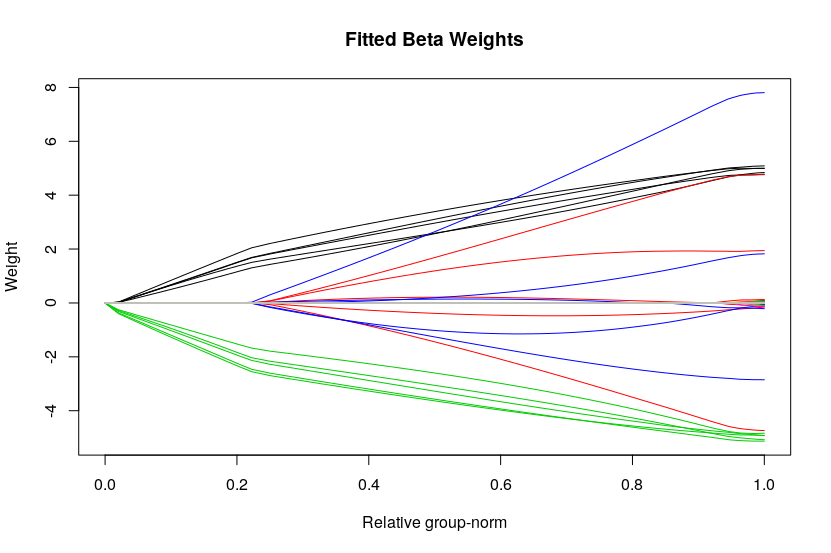
\includegraphics[scale=0.5]{fitted_beta_weights.png}
\caption{Covariate weights against relative group norm. Covariates colored by group.}
\label{fig:colorWeights}
\end{figure}

We can see that there are four active groups (all other groups remain 0 for all values and are hidden on the x-axis): black, green, red and blue. By comparing this graph with the true beta in the code above, we can get a measure of how the algorithm is performing across the various lambda values.

The black group (which we see has 5 members) quickly becomes active as lambda is decreased, and eventually all values settle at a value of 5. This is evidently the first group, which was set to five 5's. Similarly, the green group becomes active and converges to five $-5$'s; this is third group. The other two groups are active but have predictors that are 0--we can see that the red group, for instance, has a 5, a 2, and a $-5$, and must be the second group.

From comparing this output graph with the true $\beta$, with which the data was generated, one might ask what the optimal $\lambda$, is, which recovers the true structure. In this case, it appears the small end of the lambda path results in the most accurate estimates.


\section{Comparison}

First we will compare the two algorithms within the sparsegl function, threestep and fourstep, for both accuracy and speed. Then, we compare our package with two other competing packages, the \pkg{SGL} package (which performs sparse group lasso, without predictor-discarding rules) and the \pkg{gglasso} package (which only performs group lasso, but uses predictor-discarding rules). Since the main contribution of this package is a fast algorithm for sparse group lasso, we pay particular attention to the speed difference between our algorithms and SGL.

For all comparisons, we use the \texttt{R} package \pkg{microbenchmark}, which compares two or more operations by performing them repeatedly (100 for our analysis) and collecting the times to perform each operation.

\begin{figure}[tb!]
\centering
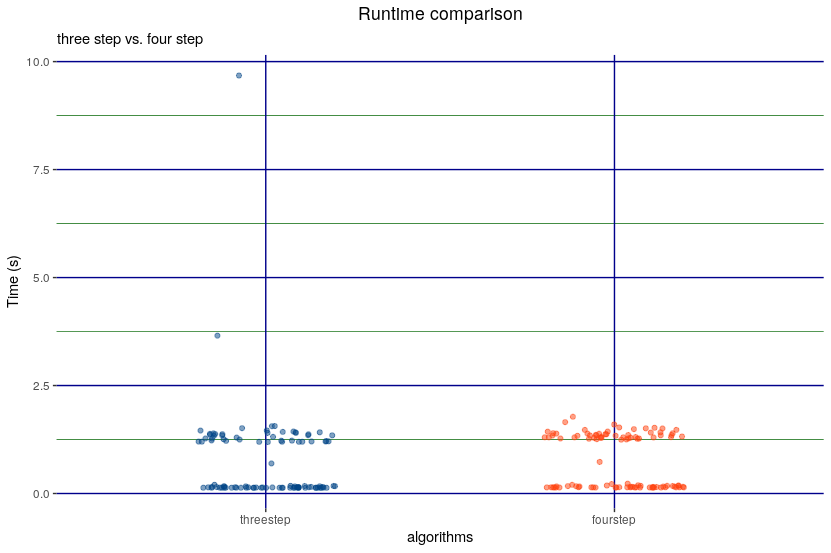
\includegraphics[scale=0.5]{threefour2.png}
\caption{A graph comparing the run-times of the threestep and fourstep algorithms.}
\label{fig:threevsfour}
\end{figure}


We can see that there is not a big difference in the time it takes to perform the threestep algorithm vs the fourstep algorithm. This is possibly a result of the simulated data used, and we believe that for some large datasets, the fourstep algorithm will outperform the threestep.

Next, we compare our package with the gglasso package, which performs regular group lasso. For this comparison we set $\alpha$ to be zero in our algorithm, so that it also performs regular group lasso. 

\begin{figure}[tb!]
\centering
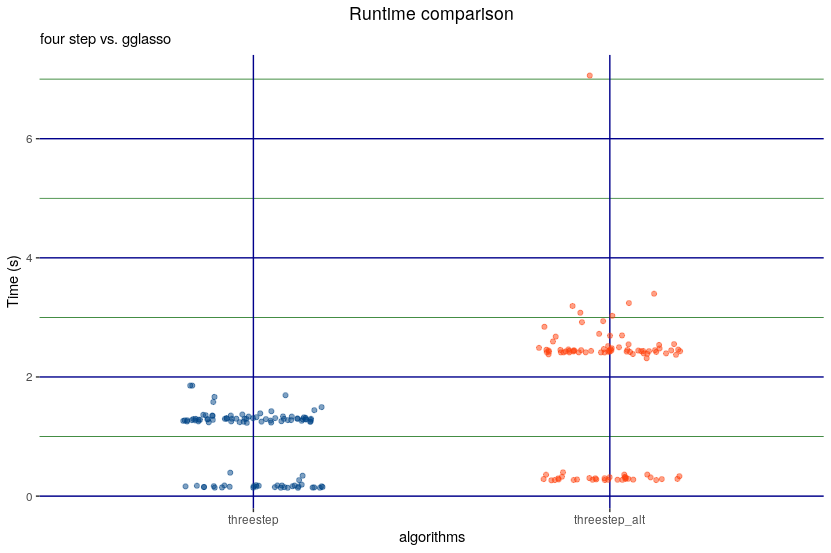
\includegraphics[scale=0.5]{fourgglasso2.png}
\caption{A graph comparing the run-times of the fourstep algorithm with the gglasso package. The fourstep algorithm is slightly faster.}
\label{fig:1fourvsgglasso}
\end{figure}

We see that our package actually outperforms gglasso, even though the gglasso incorporates a similar strong rule, and is overall very close to our threestep algorithm. This gives evidence that the fourstep algorithm can outperform the threestep in at least some circumstances. So even without considering the added functionality of sparsegl to incorporate sparseness, our sparsegl algorithm seems to be an improvement on the gglasso package for performing group lasso.

Finally, we look at the only other existing package that performs sparse group lasso, the SGL package.


\begin{figure}[tb!]
\centering
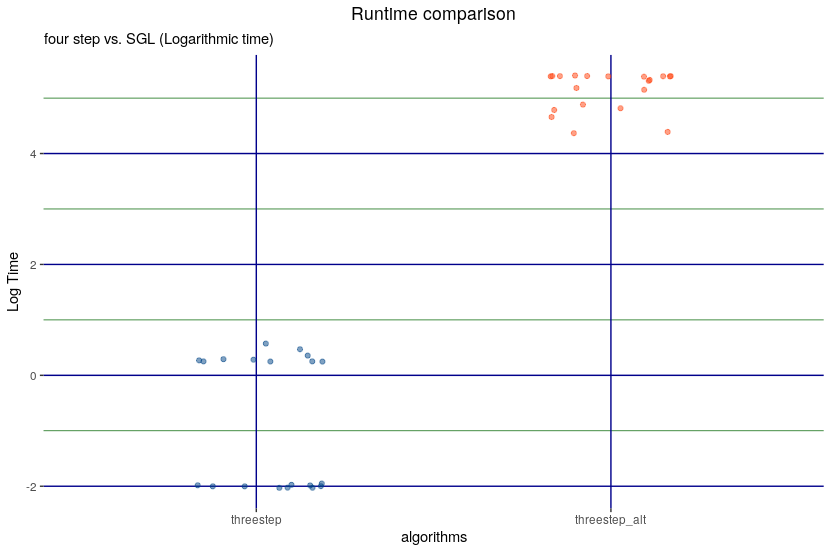
\includegraphics[scale=0.5]{fourSGL2.png}
\caption{A graph comparing the run-times of the fourstep algorithm with the SGL package. The fourstep algorithm is substantially faster than SGL in performing sparse group lasso.}
\label{fig:fourvsSGL}
\end{figure}


Here we see that our fourstep algorithm is substantially faster than SGL in performing sparse group lasso. In fact, we needed to decrease the number of times that microbenchmark ran the two algorithms, since the default of 100 tests was too much for this computer, it did not finish the job in an hour.

Recall the dataset we used for these comparisons, with $n=100$ and $p=200$. It is clear that SGL cannot be used for very large datasets, and thus the sparsegl package represents real progress.


We also compare the actual output, in particular the beta matrix, to confirm that they are arriving at the same answers. For this comparison, the lambda path is about the same, but for the other packages (gglasso, SGL), the lambda path will in general be different, so some care must be taken in comparing the beta matrices.

\section{Conclusion}


Putting this here in case I screw up \citep{tibshirani2012strong}

Then I want to put this \citep{yang2015fast} here.

And finally I recall the work of \citep{simon2013sparse} for the people.

\begin{algorithm}
  \caption{Three-step Algorithm\label{alg:kalman}}
  \begin{algorithmic}
    \STATE {\bf Input:} $\lambda_0,\ \lambda_1,\ \dots$, $\mathcal{E}$, $\mathcal{A}$
    \STATE Set $\mathcal{E}$ and $\mathcal{A}$ to $\emptyset$ \COMMENT{Step 0}
    \FOR{$i=1$ to  $n$}
    \STATE $\begin{aligned} x_{i}
      &\leftarrow d + T x_{i-1|i-1}, & P_i &\leftarrow Q + T P_{i-1|i-1}
      T^\top\end{aligned}$ \COMMENT{Predict current state}
    \STATE $\begin{aligned}\widetilde{y}_i
      &\leftarrow c + Z  x_i, & F_i &\leftarrow G + Z P_i
      Z^\top\end{aligned}$ \COMMENT{Predict current observation}
    \STATE $\begin{aligned}v_i&\leftarrow y_i-\widetilde{y}_i& K_i&
      \leftarrow P_i Z^\top F^{-1}\end{aligned}$ \COMMENT{Forecast error and 
    Kalman gain}
    \STATE $\begin{aligned} x_{i|i}
      &\leftarrow  x_i + K_i v_i, & P_{i|i} &\leftarrow P_i - P_iZ^\top
      K_i\end{aligned}$ \COMMENT{Update}
    \STATE $\ell(\theta) = \ell(\theta) -v_i^\top F^{-1}v_i - \log(|F_i|)$
    \ENDFOR
    \RETURN $\widetilde{Y}=\{\widetilde{y}_i\}_{i=1}^n,\  x=\{ x_i\}_{i=1}^n,\
    \widetilde{X}=\{x_{i|i}\}_{i=1}^n,\ P=\{P_i\}_{i=1}^n,\
    \widetilde{P}=\{P_{i|i}\}_{i=1}^n,\ \ell(\theta)$
  \end{algorithmic}
\end{algorithm}

\bibliographystyle{plainnat}
\bibliography{refs.bib}

\end{document}